\section{Bias and Variance}

Bias and variance are two sources of error in a machine learning model. 

A \textbf{simple model} is one with limited capacity to fit the data — for example, a linear model with few features or a shallow decision tree. It makes strong assumptions and cannot capture complex patterns. These models are easier to train and interpret but may underfit. A \textbf{complex model}, on the other hand, has higher capacity — such as deep neural networks or decision trees with many branches. It can capture subtle patterns in the data and fit it very closely. However, this makes it prone to overfitting, especially when the training data is noisy or limited.

\textbf{Bias} is the error from wrong assumptions in the learning algorithm. A model with high bias pays little attention to the training data and oversimplifies the model. This can lead to underfitting. \textbf{Variance} is the error from sensitivity to small fluctuations in the training set. A model with high variance learns noise in the training data as if it were true signal. This can lead to overfitting.

\begin{center}
\begin{tabular}{|c|c|c|}
\hline
\textbf{Model Type} & \textbf{Bias} & \textbf{Variance} \\
\hline
Simple Model & High & Low \\
\hline
Complex Model & Low & High \\
\hline
\end{tabular}
\captionof{table}{Bias and Variance in Simple vs Complex Models}
\end{center}

\subsection{The Tradeoff}

Both bias and variance affect the overall error, measured by the mean square error (MSE). The MSE can be broken down as
\[
\mathbb{E}\left[(\hat{f}(\mathbf{x}) - f(\mathbf{x}))^2\right] = \underbrace{(\mathbb{E}[\hat{f}(\mathbf{x})] - f(\mathbf{x}))^2}_{\text{Bias}^2} + \underbrace{\mathbb{E}[(\hat{f}(\mathbf{x}) - \mathbb{E}[\hat{f}(\mathbf{x})])^2]}_{\text{Variance}} + \underbrace{\sigma^2}_{\text{Irreducible error}}
\]

The test error as a function of model complexity typically follows a \textbf{U-shaped curve}. This shape reflects the tradeoff between bias and variance as we increase model complexity.

When the model is too simple (low complexity), it makes strong assumptions about the data and fails to capture patterns. This results in high \textbf{bias} and low \textit{variance}. The model underfits. As we increase complexity, the bias decreases — the model starts fitting the data better. Initially, this also reduces the total error. However, beyond a certain point, increasing complexity starts to hurt: the model becomes too sensitive to the training data and begins to capture noise. This leads to high \textit{variance} and low \textit{bias}, but overall error increases again. The model overfits.

So, the total test error has a minimum at some intermediate level of complexity, the \textbf{sweet spot}, where bias and variance are balanced.


\begin{figure}[h!]
\centering
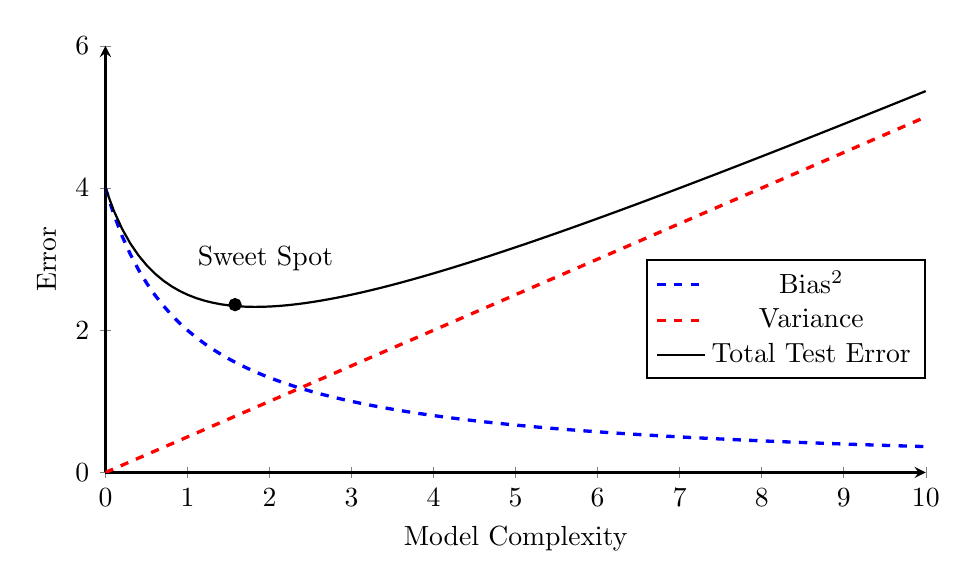
\begin{tikzpicture}
\begin{axis}[
    width=12cm,
    height=7cm,
    xlabel={Model Complexity},
    ylabel={Error},
    axis lines=left,
    legend style={at={(1,0.5)}, anchor=north east},
    domain=0:10,
    samples=100,
    ymin=0, ymax=6,
    xmin=0, xmax=10,
    thick
]

% Bias^2 curve
\addplot[blue, dashed, very thick] {4 / (x + 1)};
\addlegendentry{Bias\(^2\)}

% Variance curve
\addplot[red, dashed, very thick] {0.5 * x};
\addlegendentry{Variance}

% Total Error
\addplot[black, thick] {4 / (x + 1) + 0.5 * x};
\addlegendentry{Total Test Error}

% Sweet spot point
\addplot[
    mark=*,
    only marks,
    mark options={fill=black}
] coordinates {(1.58,2.36)};

% Detached label for sweet spot
\node at (axis cs:1,3) [anchor=west] {Sweet Spot};


\end{axis}
\end{tikzpicture}
\caption{The U-shaped nature of test error due to the bias–variance tradeoff}
\end{figure}
